\section{Indoor Location}\label{sec:designindoorlocation}
In this project, a solution for pointing at a controllable device, \eg a lamp, is proposed. 
In order to determine which device the user points at, 
and thereby intends to control, 
it is necessary to determine the locations of the devices in the system, 
relative to the user. 
We must thus know the location of the user, 
and his controllable devices along with the orientation of the user.

The orientation of the user can be retrieved from any device possessing a magnetometer. 
We found that 49 devices in Vandrico's database contain the magnetometer component. 
Given the orientation of the user, his location and the location of a controllable device, 
we can calculate if the user is looking at, 
or in the direction of, the controllable device.
We also need to define a visibility range, \ie a range that constitutes the area in which items are visible to the system. This range can be specified (in degrees) as $r = o \pm e$, where $r$ is the visibility range, $o$ is the orientation of the user and $e$ is the distance between $o$ and the edges of $r$.
\Cref{fig:visibilityangle} illustrates this. 
In this figure, the user's orientation is \var{o1}, 
and there are two devices with orientations \var{o2} and \var{o3}. 
An orientation in degrees is between \num{0} and \num{360}. 
To determine whether a device with orientation \var{o2} is within the visibility range, 
it is a simple matter of calculating whether \var{o2} is greather than $\var{o1}-\var{e}$ and smaller than $\var{o1}+\var{e}$, with some exceptions when the visibility range spans the gap between 359\degree and 0\degree.

\begin{figure}[!htb]
    \centering
    \def\svgwidth{0.6\textwidth}
    \import{drawings/}{drawings/visibilityangle.pdf_tex}
    \caption{Finding objects in the visibility range. Device 1 is within the range, but Device 2 is not.}
\label{fig:visibilityangle}
\end{figure}

The focus of this project is not to position devices, 
and as such it was not the intention to spend time developing an entire solution for positioning devices indoors. 
Instead it was desired to find an existing product, 
that could be used to facilitate indoor positioning.
The solution should be available in the early phases of the project, 
in order to start building the system based on the solution for positioning.

As the target group of the project is consumers, 
and not businesses with big budgets, 
it is desired that the price of the technology used for indoor positioning is kept at a minimum. 
This includes the price for any device, 
that may have to be installed on each controllable device in order to position it.

It is assumed that users already own one or more devices that fit within the concept of Internet of Things, 
and are early adapters of such technology. 
However, it easy to imagine that this project can be used in an office environment, 
where employees of varying technological expertise work or in health care. 
Therefore users may have a varying degree of technological expertise, 
and it should be easy to extend the solution with new controllable devices.

Naturally the accuracy of the solution used for indoor positioning plays an important part. 
\Cref{fig:indoor-positioning:incorrect} shows the consequence of an incorrect location. 
If a lamp is estimated to be at another location that it is actually located, 
the user must point to an incorrect location in order to control the lamp.
Furthermore if the estimate is too wide, 
\ie the given area in which the lamp is located is very big, 
there is a greater risk that locations overlap. 
Overlapping locations causes a complexity, 
as it is necessary to determine which device the user desires to control, 
if he points at the overlap as visualized in \Cref{fig:indoor-positioning:overlap}.

\begin{figure}[!htb]
    \centering
    \begin{minipage}[t]{0.45\textwidth}
        \centering
        
\includegraphics[width=0.6\textwidth]{images/incorrect-positioning-estimate.png}
        \caption{Incorrect location estimate. The estimate is visualized as a striped circle.}
        \label{fig:indoor-positioning:incorrect}
    \end{minipage}\qquad
    \begin{minipage}[t]{0.45\textwidth}
        \centering
        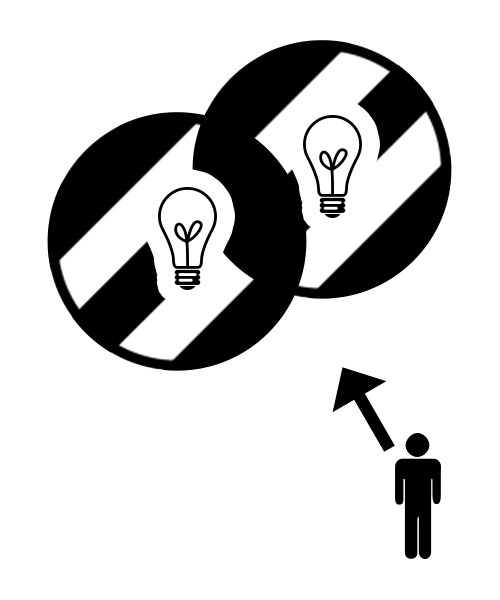
\includegraphics[width=0.6\textwidth]{images/positioning-overlap.png}
        \caption{Overlap of estimated positions. The estimates are visualized as a striped circle.}
        \label{fig:indoor-positioning:overlap}
    \end{minipage}
\end{figure}


\subsection{Analysis of Potential Existing Solution}
This section will be an analysis of commercialized products that offer indoor location.
Only solutions intended for indoor positioning are considered.
GPS is not considered a potential solution as GPS is meant for outdoor positioning, 
and the location offered by GPS tend to have poor accuracy indoors.
We have chosen not to include solutions designed for larger buildings such as airports, malls or warehouses, 
as these does not provide solutions or setups for smaller areas such as rooms or houses. 

\Cref{tbl:indoor-positioning} shows the results of the analysis. 
\begin{table}[!htb]
    \begin{description}[style=multiline,leftmargin=2.5cm]
        \item[Product:] Estimote Beacons and Stickers \cite{estimote}
        \item[Availability:] Beacons and Stickers are shipping. SDKs available.
        \item[Technology:] iBeacon protocol.
        \item[Price:] \SI{99}[\$]{} for beacons. \SI{99}[\$]{} for 10 stickers, one per device to be positioned.
        \item[Ease of use:] Initial installation of beacons. Attach each sticker to device.
        \item[Accuracy:] 0.5-1 m \cite{estimote:accuracy}

        \item[Product:] Pozyx \cite{pozyx}
        \item[Availability:] Available for preorder.
        \item[Technology:] Ultra-wideband (UWB).
        \item[Price:] \$368 for anchors. \SI{123}[\$]{} for each device to be positioned, plus supported Arduino.
        \item[Ease of use:] Initial installation of anchors. One tag for each device, plus supported Arduino. Not meant for mounting.
        \item[Accuracy:] Claimed to be 10 cm. Untested. \\
        
        \item[Product:] SmartActionSLAM \cite{SASLAM}
        \item[Availability:] Android Application (research). Not commercialized.
        \item[Technology:] Smartphone sensors.
        \item[Price:] N/A.
        \item[Ease of use:] Requires modification of source code (available) to get real-time position. 
        \item[Accuracy:] Reported to have a mean error of 0.34m (only using smartphone and no external sensors).\\
        
        \item[Product:] DecaWave's DW1000 \cite{decawave}
        \item[Availability:] Available in stores. 
        \item[Technology:] Ultra-wideband (UWB)
        \item[Price:] Chips are \SI{12.50}[\$]{}, transceiver module is \SI{25}[\$]{}. Evaluation kits are available for \SI{589}[\$]{} and \SI{990}[\$]{} 
        \item[Ease of use:] No SDK and requires implementing the chips on a board yourself. 
        \item[Accuracy:] Claimed to be 10cm. 
        \end{description}
    \caption{Assessment of potential solutions for indoor positioning. Please note that all prices are converted to U.S. dollars from their respective currency. Prices include the minimum available hardware for positioning a device.}
    \label{tbl:indoor-positioning}
\end{table}

Estimote gives a solution using Bluetooth Low Energy (BLE) beacons using the iBeacon protocol. 
The beacons can be mounted on walls in a room or building, 
and then by using the signal strength of each beacon (an iBeacon feature), 
it can estimate how far away the user is. 
Estimote's solution is available as a consumer product.

Pozyx and DecaWave use a wireless radio technology known as ultra-wideband, which works much like BLE but at a different frequency. 
Like Estimote, it also requires setting up ``anchors'' and then using the signal strength to find the location. 
No easy to use consumer product is available for either of these.

SmartActionSLAM is an Android application from research done by Hardegger \etal \cite{SASLAM}. 
This solution is a lot different from most other indoor location solutions. 
It \emph{calculates} an estimated location by counting steps and estimating step length and direction. 
In theory it can be adapted to almost any smartphone, 
but requires a lot of work to adapt the released code from the research project. 

\subsection{Estimote}

Beacons are used for indoor location in this project. Estimote is one of many vendors of iBeacons. Common use cases for beacons include monitoring if the user enters a specific region of an area. This can be used to push location specific information or advertisement when a user is near a shop or even a certain product in that shop.

Estimote not only focus on typical use cases for beacons like entering a specific region, but have also specialized in indoor location of users using the beacon technology. The company developed the Estimote Indoor Location application for iOS\footnote{https://itunes.apple.com/us/app/estimote-indoor-location/id963704810} which is meant to ease configuration needed for indoor location. A user will install the beacons in a room by placing one beacon on each wall. Next the user walks along the perimeter of the room and thereby registering the location of the beacons by collecting signal strengths from the beacons and data from the phones accelerometer and/or gyroscope.
After the configuration, the application has estimated the length of and placement of walls allong with the signal strengths of each beacon.

During our tests we found that the approach for configuring the indoor locationing describe above works terribly or not at all. After configurin the room, the application would show an illustration of the registered room and we found the measurements to to be very inaccurate. The Estimote Indoor Location application was therefore abandoned for configuring a room.

\subsubsection{Configuring Rooms Programmatically}

Estimote provides Estimote Indoor Location SDK\footnote{https://github.com/Estimote/iOS-Indoor-SDK} to perform indoor locationing using beacons on iOS. The SDK provides two mechanisms for configuring a room for indoor positioning.

\begin{enumerate}
\item Using the built-in controller. The component presents the user with a guided configuration similar to the one used in the Estimote Indoor Location application.
\item Programmatically using the \texttt{ESTLocationBuilder} class.
\end{enumerate}

The built-in controller was abandoned as it uses the exact same technology as the Estimote Indoor Location application and therefore results in poor accuracy.

The \texttt{ESTLocationBuilder} lets developers configure a room programmatically by passing XY-points and an orientation to the builder. The X and Y value of each point is measured in meters. Therefore a point $(0, 0$) to $(0, 5)$ represents a horisontal line of five meters and the set of points $\{(0,0),(0,5),(5,5),(5,0)\}$ represents a room of size 5 meters by 5 meters.

\begin{listing}
\begin{swiftcode}
        let locationBuilder = ESTLocationBuilder()
        locationBuilder.setLocationBoundaryPoints([
            ESTPoint(x: 0.cmToMeter(), y: 0.cmToMeter()),
            ESTPoint(x: 537.cmToMeter(), y: 0.cmToMeter()),
            ESTPoint(x: 537.cmToMeter(), y: 60.cmToMeter()),
            ESTPoint(x: 690.cmToMeter(), y: 60.cmToMeter()),
            ESTPoint(x: 690.cmToMeter(), y: 385.cmToMeter()),
            ESTPoint(x: 0.cmToMeter(), y: 385.cmToMeter()),
        ])
        
        let ice3 = "dec18deac0c5"
        let blueberry3 = "f13173ad3185"
        let ice2 = "d470d26d33f3"
        let mint3 = "e6d39dee79c9"
        
        locationBuilder.addBeaconIdentifiedByMac(blueberry3, atBoundarySegmentIndex: 0, inDistance: 422.cmToMeter(), fromSide: .RightSide)
        locationBuilder.addBeaconIdentifiedByMac(ice3, atBoundarySegmentIndex: 3, inDistance: 222.cmToMeter(), fromSide: .RightSide)
        locationBuilder.addBeaconIdentifiedByMac(mint3, atBoundarySegmentIndex: 4, inDistance: 335.cmToMeter(), fromSide: .LeftSide)
        locationBuilder.addBeaconIdentifiedByMac(ice2, atBoundarySegmentIndex: 5, inDistance: 165.cmToMeter(), fromSide: .LeftSide)
        locationBuilder.setLocationOrientation(130)
        locationBuilder.setLocationName("Gros Stue")
        
        let location = locationBuilder.build()
\end{swiftcode}
\caption{Example usage of the \texttt{ESTLocationBuilder} class.}
\label{lst:estlocationbuilder}
\end{listing}

Listing \ref{lst:estlocationbuilder} shows how we used the \texttt{ESTLocationBuilder} to create a model of a real world living room. The resulting model is illustrated in figure \ref{fig:estlocationbuilder-livingroom}.

The builder is configured with six points that gives information about the shape of the room. Next, the beacons are added to the walls of the room. Beacons are added with the identifier of the beacon. Lastly the orientation of the room relative to north and the name of the room is set. When the room has been configured it can be stored on the users Estimote account using the Estimote SDK.

Using the \texttt{ESTLocationBuilder} to model a room reduces any uncertainties in estimating the users location caused by an imprecise model of the room.

\begin{figure}
\centering
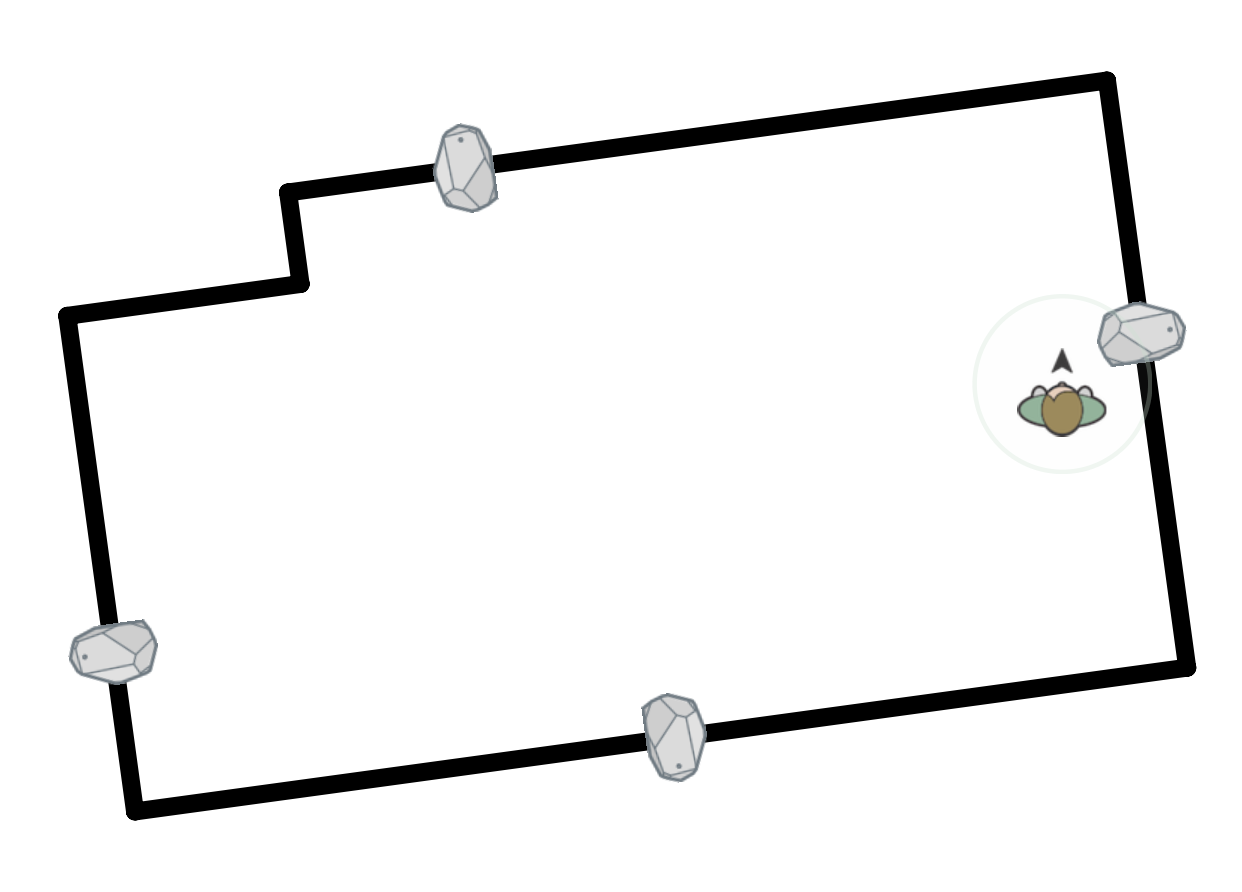
\includegraphics[width=0.33\textwidth]{images/living-room}
\caption{Model created using the \texttt{ESTLocationBuilder} as shown in listing \ref{lst:estlocationbuilder}. Note that the model is rotated accordingly to the orientation of the room and the position of north relative to the user.}
\label{fig:estlocationbuilder-livingroom}
\end{figure}

\subsubsection{Ranging in the Background}

There are two distinct ways of locating a user when using iBeacon \cite{estimote:monitoring-ranging}.

\begin{itemize}
\item Region monitoring is performed to check if a user enters or leaves a specific region. A region is a geofence, a virtual perimeter around some location. Such region could be used to check if a user arrives or leaves his house, his workplace or if he is nearby a shop encapsulated in a geofence. Regions are useful for performing simple home automation, e.g. turn the lights on when the user arrives at home and turn them off when they leave.
\item Ranging is more granular than region monitoring and is used to continuously retrieve the set of beacons in range along with an estimated distance to them based on the signal strengths. Ranging is used to get a granular user position.
\end{itemize}

According to both Apple and Estimote it is preferred that ranging is only performed while the application is in the foreground, that is, the application is on the screen and the user is likely to interact with the application. The reason for this is that ranging for beacons can have a negativ impact on the battery life where as the region monitoring do not use as much battery power.

While Apple and Estimote advise agains performing beacon ranging in the background, it is possible \cite{apple:monitoring-ibeacon} \cite{estimote:monitoring-ranging}.

%%% Local Variables:
%%% mode: latex
%%% TeX-master: "../../master"
%%% TeX-command-extra-options: "-shell-escape"
%%% End:

%%% Local Variables:
%%% mode: latex
%%% TeX-master: "../../master"
%%% TeX-command-extra-options: "-shell-escape"
%%% End:
